\documentclass[10pt,a4paper]{article}
\usepackage[utf8]{inputenc}
\usepackage[spanish]{babel}
\usepackage{amsmath}
\usepackage{amsfonts}
\usepackage{amssymb}
\usepackage{enumitem}
\usepackage{hyperref} 
\usepackage{graphicx}
\usepackage{appendix}
\usepackage[margin=0.6in]{geometry}
\hypersetup{pdftex,colorlinks=true,allcolors=black}
\hypersetup{
    pdftitle={},
    pdfauthor={Pablo Riutort Grande},
    pdfsubject={},
    bookmarksnumbered=true,     
    bookmarksopen=true,         
    bookmarksopenlevel=1,       
    colorlinks=true,            
    pdfstartview=Fit,           
    pdfpagemode=UseOutlines,    % this is the option you were lookin for
    pdfpagelayout=TwoPageRight
}
\usepackage{listings}
\usepackage{xcolor}
\usepackage{hypcap}
\definecolor{codegreen}{rgb}{0,0.6,0}
\definecolor{codegray}{rgb}{0.5,0.5,0.5}
\definecolor{codepurple}{rgb}{0.58,0,0.82}
\definecolor{backcolour}{rgb}{0.95,0.95,0.92}
\usepackage{caption}
\usepackage{subcaption}
\lstdefinestyle{mystyle}{
    backgroundcolor=\color{backcolour},   
    commentstyle=\color{codegreen},
    keywordstyle=\color{magenta},
    numberstyle=\tiny\color{codegray},
    stringstyle=\color{codepurple},
    basicstyle=\ttfamily\footnotesize,
    breakatwhitespace=false,         
    breaklines=true,                 
    captionpos=b,                    
    keepspaces=true,                 
    numbers=left,                    
    numbersep=5pt,                  
    showspaces=false,                
    showstringspaces=false,
    showtabs=false,                  
    tabsize=2
}
\usepackage{tabulary}
\usepackage{colortbl}
\lstset{style=mystyle}
\usepackage{xparse}
\NewDocumentCommand{\codeword}{v}{%
\texttt{{#1}}
}
\author{Pablo Riutort Grande}
\title{Biometría \\\vspace{0.3cm}PEC 2\\ \vspace{1cm}\textbf{Reconocimiento de las personas por la huella dactilar}}

\begin{document}
\maketitle

\pagebreak

\listoffigures
\listoftables
\pagebreak
\section{}
\subsection{}
Para este ejercicio se han generado las huellas de un dedo índice de clases arco, lazo izquierdo, lazo derecho, arco en forma de pico o tienda y espiral. En cada huella se han identificado 2 minutias distintas, bifuración y terminal, marcadas de color blanco. Las espirales se han marcado en rojo, los lazos en azul y los deltas en amarillo.

\begin{figure}[h!]
\centering
\begin{subfigure}{.5\textwidth}
  \centering
  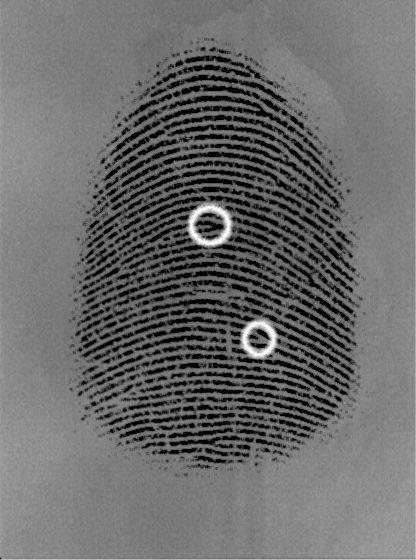
\includegraphics[width=.7\linewidth]{1/arch.png}
  \caption{Huella de clase arco}
  \label{fig:arch}
\end{subfigure}%
\begin{subfigure}{.5\textwidth}
  \centering
  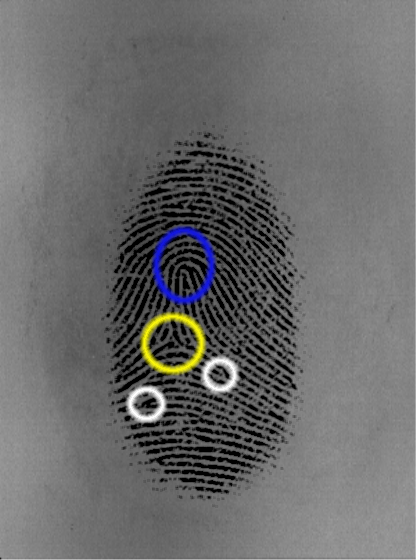
\includegraphics[width=.7\linewidth]{1/tented_arch.png}
  \caption{Huella de clase arco en forma de pico o tienda}
  \label{fig:tented_arch}
\end{subfigure}

\begin{subfigure}{.5\textwidth}
  \centering
  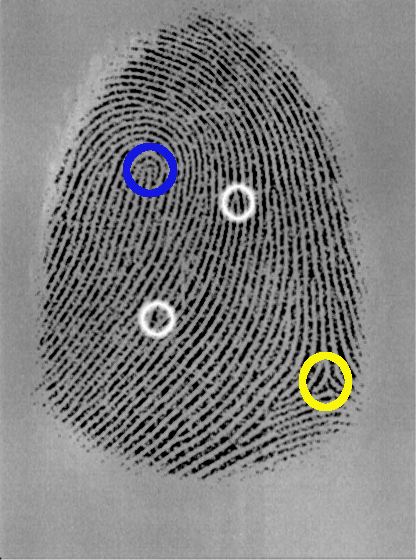
\includegraphics[width=.7\linewidth]{1/left_loop.png}
  \caption{Huella de clase de lazo izquierdo}
  \label{fig:left_loop}
\end{subfigure}%
\begin{subfigure}{.5\textwidth}
  \centering
  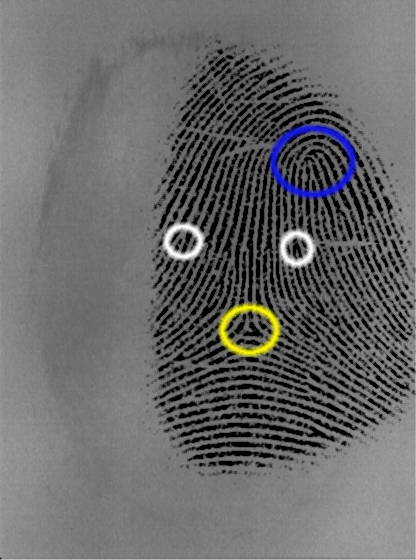
\includegraphics[width=.7\linewidth]{1/right_loop.png}
  \caption{Huella de clase de lazo derecho}
  \label{fig:right_loop}
\end{subfigure}
	\caption{Huellas generadas}
\end{figure}

\begin{figure}[h!]
  \centering
  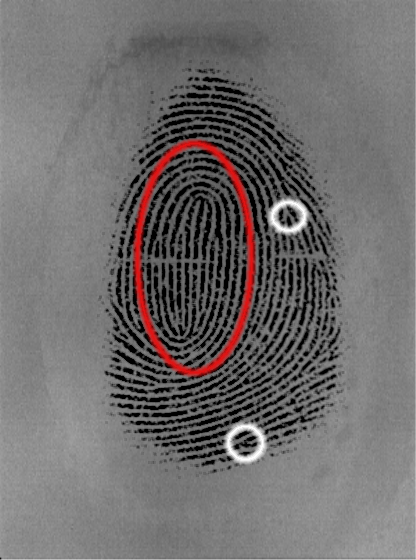
\includegraphics[scale=0.6]{1/whorl.png}\\
  \caption{Huella de clase espiral}
  \label{fig:whirl}
\end{figure}

\pagebreak

\subsection{}
Para este ejercicio se han generado dos huellas del pulgar de mismas características excepto en \textit{Ridge density}. Estas huellas han sido analizadas con el software de edición de imagen Gimp y con la herramienta \textit{Measure} se han obtenido las distancias en píxeles entre cordilleras de ambas imágenes, siendo de 3 píxeles para el \textit{Ridge density} mínimo y 6 píxeles para el \textit{Ridge density} máximo.
\begin{figure}[h!]
\centering
\begin{subfigure}{.5\textwidth}
  \centering
  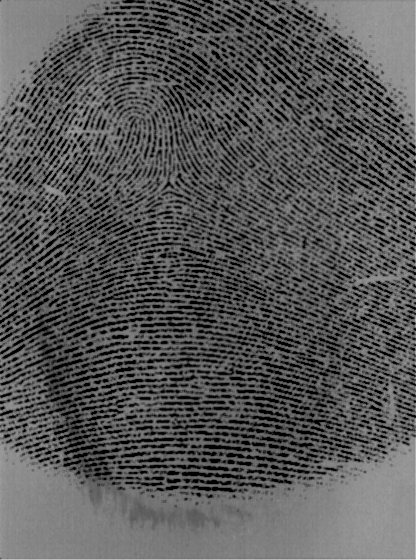
\includegraphics[width=.7\linewidth]{1.2/min_original.png}
  \caption{Huella dactilar generada con \textit{Ridge Density} mínima}
  \label{fig:min_ridge}
\end{subfigure}%
\begin{subfigure}{.5\textwidth}
  \centering
  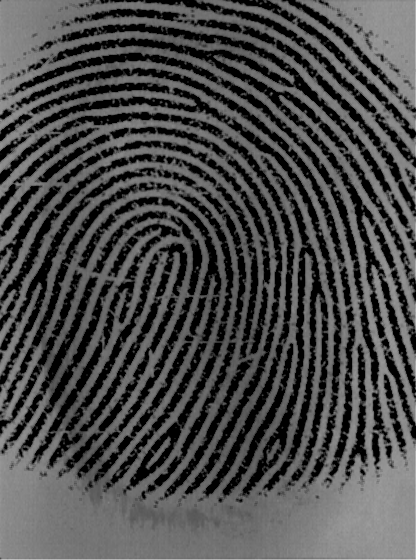
\includegraphics[width=.7\linewidth]{1.2/max_original.png}
  \caption{Huella dactilar generada con \textit{Ridge Density} máxima}
  \label{fig:max_ridge}
\end{subfigure}
\caption{Imágenes generadas con distintas \textit{Ridge Density}}
\label{fig:ridge}
\end{figure}

\begin{figure}[h!]
  \centering
  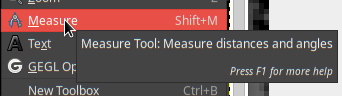
\includegraphics[width=.7\linewidth]{1.2/measure.png}
  \caption{Herramienta utilizada para este ejercicio del editor de imágenes Gimp}
  \label{fig:measure}
\end{figure}

\begin{figure}[h!]
\centering
\begin{subfigure}{.5\textwidth}
  \centering
  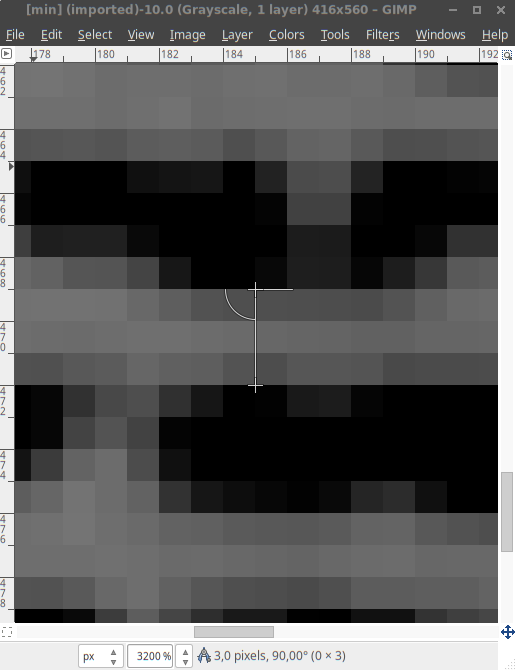
\includegraphics[width=.7\linewidth]{1.2/min.png}
  \caption{Distancia de 3 píxeles en \textit{Ridge Density} mínima}
  \label{fig:min_ridge}
\end{subfigure}%
\begin{subfigure}{.5\textwidth}
  \centering
  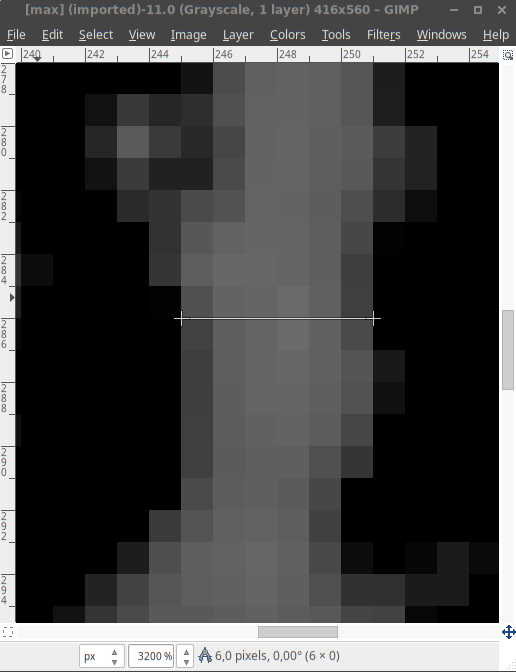
\includegraphics[width=.7\linewidth]{1.2/max.png}
  \caption{Distancia de 6 píxeles en \textit{Ridge Density} máxima}
  \label{fig:max_ridge}
\end{subfigure}
\caption{Cálculo de las distancias entre cordilleras}
\label{fig:measurements}
\end{figure}

\pagebreak

\subsection{}
El \textit{noise} en los dos sensores tienen un significado diferente. Los sensores ópticos utilizan la luz para adquirir la imagen, las cordilleras están en contacto con la superficie del sensor y los valles no, por tanto, la luz que se refleja en el dedo es absorvida por las cordilleras reflejada en los valles. Por tanto, un sensor con ruído en este contexto podría significar que la luz no está del todo bien reflejada en la huella (suciedad en el sensor, en el dedo, etc).\\
En cambio, los sensores capacitivos son un tipo de sensores de estado sólido que detectan diferencias de cargas eléctricos entre cordilleras y valles poniendo el dedo en contacto con una placa de microcondensadores; los cambios de capacitancia entre cordillera y valle medidos son traducidos a voltage. El ruido, en este contexto, se refiere al producido por las celdas de microcondensadores, los circuitos de sensores o al propio cuerpo humano en las capacitancias \cite{cmos}.\\

En caso de que la persona tuviera los dedos sucios aplicaría un sensor de tipo capacitivo debido que este tipo de sensores son más tolerantes a ese tipo de interferencias ya que funcionan con diferencias de cargas eléctricas y no con una imagen que puede ser susceptible de verse alterada por un dedo mojado o un cristal sucio.
\pagebreak
\begin{figure}[h!]
\centering
\begin{subfigure}{.5\textwidth}
  \centering
  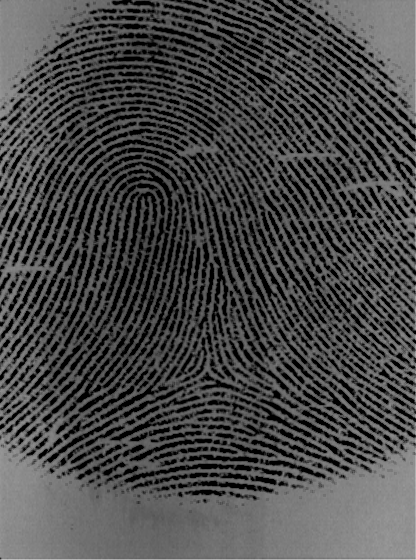
\includegraphics[width=.7\linewidth]{1.3/capacitive_min.png}
  \caption{Huella en sensor capacitivo con ruido al mínimo}
  \label{fig:capac_min}
\end{subfigure}%
\begin{subfigure}{.5\textwidth}
  \centering
  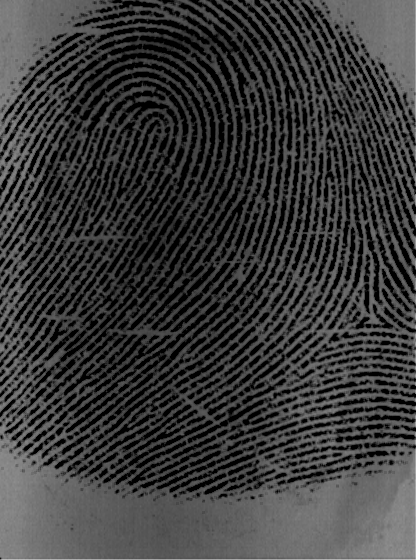
\includegraphics[width=.7\linewidth]{1.3/capacitive_max.png}
  \caption{Huella en sensor capacitivo con ruido al máximo}
  \label{fig:capac_max}
\end{subfigure}

\begin{subfigure}{.5\textwidth}
  \centering
  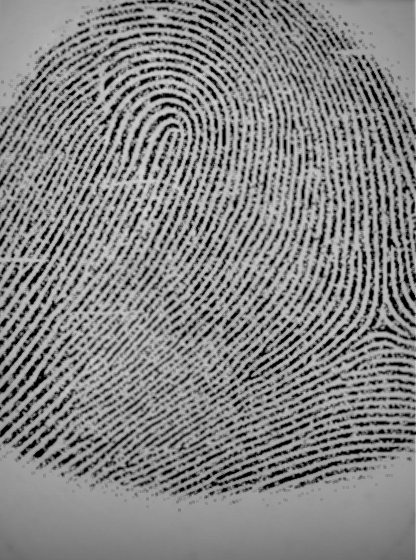
\includegraphics[width=.7\linewidth]{1.3/optical_min.png}
  \caption{Huella en sensor óptico con ruido al mínimo}
  \label{fig:opt_min}
\end{subfigure}%
\begin{subfigure}{.5\textwidth}
  \centering
  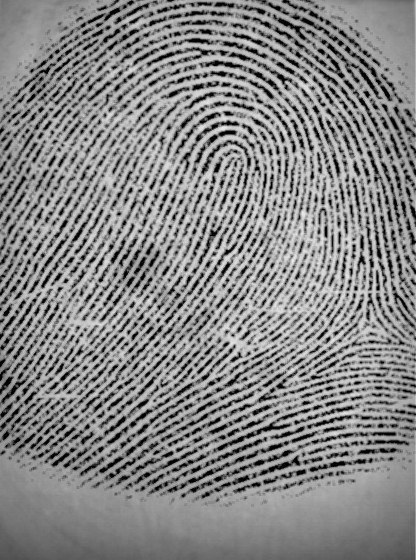
\includegraphics[width=.7\linewidth]{1.3/optical_max.png}
  \caption{Huella en sensor óptico con ruido al máximo}
  \label{fig:opt_max}
\end{subfigure}
\end{figure}

\pagebreak
\subsection{}

\begin{table}[htbp]
\centering
\begin{tabular}{|c|c|c|c|c|c|c|}
\hline
 & \textbf{D1} & \textbf{D2}  & \textbf{D3}  & \textbf{D4}  & \textbf{D5}  & \textbf{D6} \\ \hline
  \textbf{Clase huella} & Lazo izquierdo & Espiral & Espiral & Espiral & Espiral & Lazo derecho \\ \hline

\end{tabular}

  \caption{Clase huellas d1 a d6}
  \label{tabla:clases}
\end{table}

\begin{table}[h!]
\centering
\begin{tabular}{|c|c|c|c|c|c|c|}
\hline
 & \textbf{D1} & \textbf{D2}  & \textbf{D3}  & \textbf{D4}  & \textbf{D5}  & \textbf{D6} \\ \hline
   \textbf{D1} & \cellcolor{gray!25}607 & 6 & 1 & 5 & 1 & 3 \\ \hline
   \textbf{D2} & 6 & \cellcolor{gray!25}604 & 3 & 17 & 3 & 3 \\ \hline
   \textbf{D3} & 1 & 3 & \cellcolor{gray!25}667 & 6 & 2 & 1\\ \hline
   \textbf{D4} & 4 & 17 & 6 & \cellcolor{gray!25}655 & 3 & 2 \\ \hline
   \textbf{D5} & 1 & 3 & 2 & 3 & \cellcolor{gray!25}773 & 1 \\ \hline
   \textbf{D6} & 2 & 3 & 1 & 2 & 1 & \cellcolor{gray!25}501 \\ \hline

\end{tabular}

  \caption{Medidas de similitud}
  \label{tabla:medidas}
\end{table}

La pareja de huellas diferentes con mayor similtud es D2 y D4 con 17 puntos.\\
Dados los resultados tan bajos de similitud obtenidos entre las huellas dactilares de la misma clase y que solo tenemos una clase que contenga más de una huella no creo que se pueda concluir en que las huellas dactilares de la misma clase tienden a tener mayor similitud.
\section{}

\subsection{}

\begin{enumerate}[label=\textbf{\alph*)}]
\item \begin{figure}
  \centering
  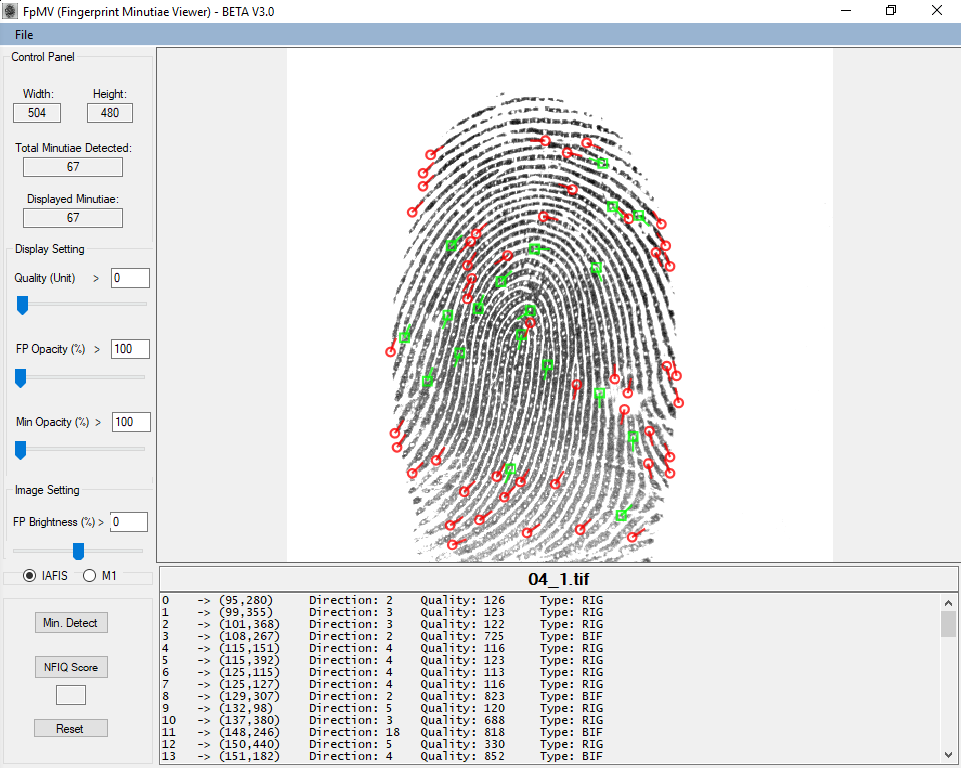
\includegraphics[width=.9\linewidth]{2_1.png}
  \caption{Información generada por el programa FpMV}
  \label{fig:FpMV}
\end{figure}

El programa FpMV genera un total de 5 columnas, todas ellas referentes a las minutiae de la huella \ref{fig:FpMV}:
\begin{enumerate}[label=\textbf{\arabic*)}]
\item Número de minutiae.
\item Coordenada x e y de la minutiae en la imagen.
\item La dirección de la minutiae detectada. Se tra del ángulo respecto a un círculo de segmentos de 11.25 grados cuyo 0 es la vertical \cite{nist}.
\item Es la fiabilidad de la minutia detectada. Se trata de una heurística resultado de combinar el nivel de calidad y las estadísticas de los píxeles vecinos al punto de la minutiae. El rango de este número es de 0.0 a 1.0 siendo el mínimo y el máximo los valores posibles respectivamente \cite{nist}.
\item El tipo, siendo BIF una bifurcación y RIG una terminación (\textit{Ridge termination}) \cite{nist}.
\end{enumerate}
El total de minutiaes detectadas es 67.

\item La zona donde aparecen las minutiae de mayor calidad aparecen agrupadas en la parte izquierda de la huella con cierto desplazamiento hacia la parte inferior \ref{fig:good}. Las zonas de menor calidad se encuentran en los extremos de la huella, especialmente en el extremo izquierdo \ref{fig:bad}.

\begin{table}[h!]
\centering
\begin{tabular}{|c|c|c|}
\hline
 \textbf{Coordenada} & \textbf{Fiabildiad} & \textbf{Tipo}\\ \hline
 129,307 & 823 & Bifurcación\\ \hline
 148,246 & 818 & Bifurcación\\ \hline
 151,182 & 852 & Bifurcación\\ \hline
 159,281 & 904 & Bifurcación\\ \hline
 166,200 & 842 & Bifurcación\\ \hline
 166,231 & 834 & Terminal\\ \hline
 170,212 & 838 & Terminal\\ \hline
 169,178 & 819 & Terminal\\ \hline
 176,240 & 900 & Bifurcación\\ \hline
 203,191 & 827 & Terminal\\ \hline
\end{tabular}
  \caption{Las 10 minutaes con mejor fiabilidad de 4\_1}
  \label{tabla:good}
\end{table}

\pagebreak

\begin{figure}[h!]
\centering
  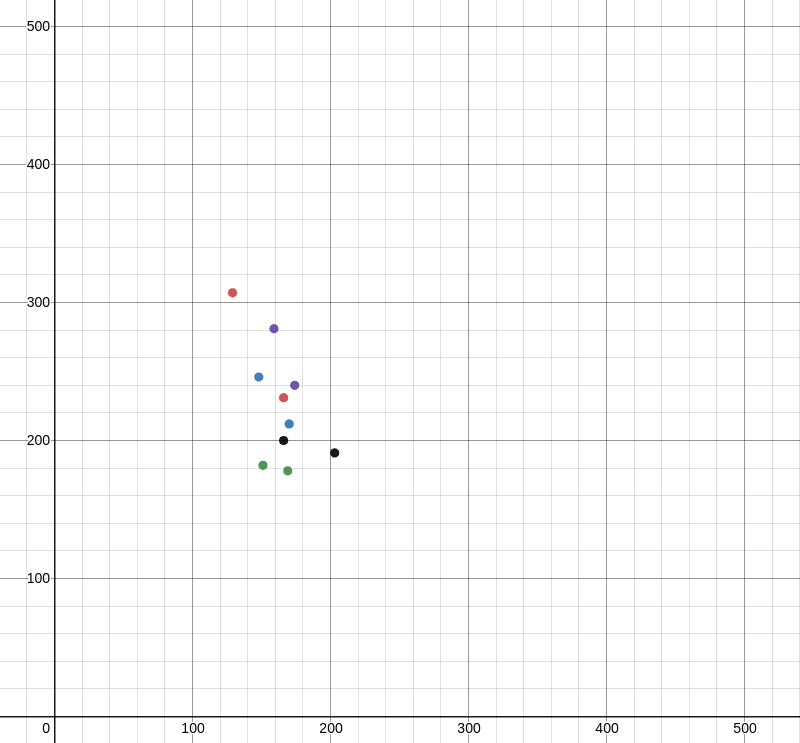
\includegraphics[width=.4\linewidth]{good.png}
  \caption{Representación gráfica de los valores de mejor fiabilidad del Cuadro \ref{tabla:good}.}
  \label{fig:good}
\end{figure}

\begin{table}[h!]
\centering
\begin{tabular}{|c|c|}
\hline
 \textbf{Coordenada} & \textbf{Fiabilidad} \\ \hline
 125,115 & 113 \\ \hline
 125,127 & 116 \\ \hline
 115,151 & 116 \\ \hline
 132,98 & 120 \\ \hline
 359,302 & 120 \\ \hline
 101,368 & 122 \\ \hline
 99,355 & 123 \\ \hline
 95,280 & 126 \\ \hline
 353,392 & 126 \\ \hline
 353,377 & 135 \\ \hline
\end{tabular}
  \caption{Las 10 minutaes con menor fiabilidad de 4\_1}
  \label{tabla:bad}
\end{table}

\begin{figure}[h!]
\centering
  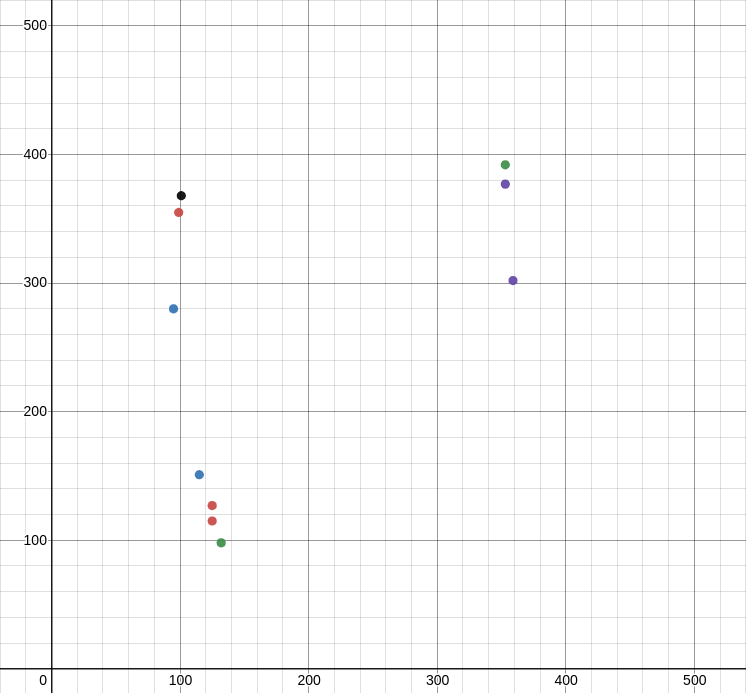
\includegraphics[width=.4\linewidth]{bad.png}
  \caption{Representación gráfica de los valores de menor fiabilidad del Cuadro \ref{tabla:bad}.}
  \label{fig:bad}
\end{figure}



\end{enumerate}

\pagebreak

\subsection{}

\begin{enumerate}[label=\textbf{\alph*)}]
\item En la figura 4\_1 el número de minutiaes de tipo bifurcación son 6 y las de tipo terminal 4 (Cuadro \ref{tabla:good}). En la figura 4\_2 el número de minutiaes de tipo de tipo bifurcación son 7 y las de tipo terminal son 6 (Cuadro \ref{tabla:good4_2}).
\begin{table}[h!]
\centering
\begin{tabular}{|c|c|c|}
\hline
 \textbf{Coordenada} & \textbf{Fiabildiad} & \textbf{Tipo}\\ \hline
 169,235 & 808 & Terminal\\ \hline
 178,172 & 833 & Bifurcación\\ \hline
 186,261 & 861 & Terminal\\ \hline
 191,218 & 841 & Terminal\\ \hline
 196,189 & 890 & Bifurcación\\ \hline
 196,201 & 874 & Terminal\\ \hline
 204,224 & 883 & Bifurcación\\ \hline
 211,289 & 848 & Terminal\\ \hline
 215,296 & 854 & Bifurcación\\ \hline
 231,183 & 804 & Bifurcación\\ \hline
 259,176 & 814 & Bifurcación\\ \hline
 270,270 & 880 & Bifurcación\\ \hline
 288,125 & 800 & Terminal\\ \hline
 
\end{tabular}
  \caption{Las 10 minutaes con mejor fiabilidad de 4\_2}
  \label{tabla:good4_2}
\end{table}

\begin{figure}[h!]
\centering
  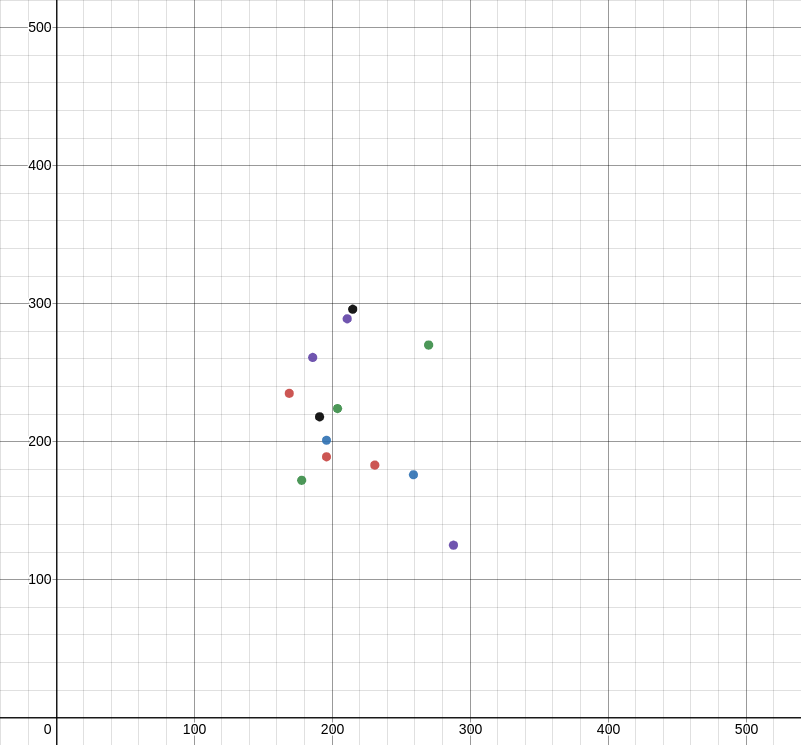
\includegraphics[width=.4\linewidth]{4_2.png}
  \caption{Representación gráfica de los valores de mayor fiabilidad del Cuadro \ref{tabla:good4_2}.}
  \label{fig:bad}
\end{figure}
\item El criterior de emparejamiento para esta comparación ``a ojo'' será el de buscar las minutiaes con coordenadas más cercanas entre sí y que FpMV haya etiquetado como minutiae del mismo tipo (terminal o bifurcación).
\begin{figure}[h!]
\centering
  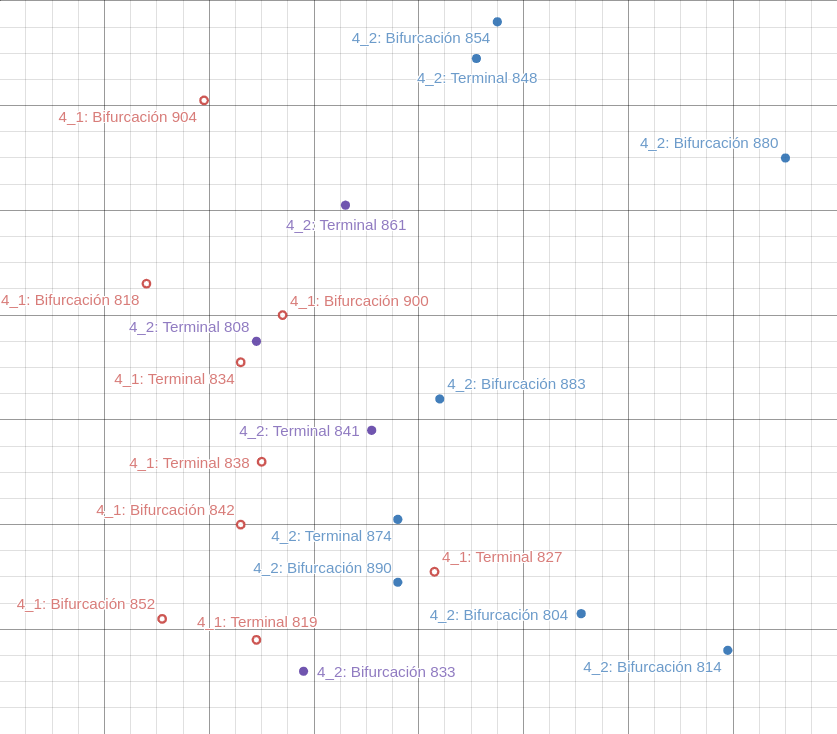
\includegraphics[width=.4\linewidth]{2_2.png}
  \caption{Representación gráfica de los valores de mayor fiabilidad de ambas figuras más próximos entre ellos}
  \label{fig:minut_compare}
\end{figure}

\begin{table}[h!]
\centering
\begin{tabular}{|c|c|c|c|c|c|}
\hline
 \textbf{\textit{m}} &\textbf{Coordenada 4\_1} & \textbf{Dirección} & \textbf{Tipo} & \textbf{Coordenada 4\_2} & \textbf{Dirección}\\ \hline
  1 & 166,231 & 2 & Terminal & 169,235 & 18 \\ \hline
  2 & 170,212 & 19 & Terminal & 191,218 & 3 \\ \hline
  3 & 203,191 & 21 & Terminal & 196,201 & 19\\ \hline
  4 & 166,200 & 3 & Bifurcación & 196,189 & 4 \\ \hline
  5 & 176,240 & 2 & Bifurcación & 204,224 & 3 \\ \hline
\end{tabular}
  \caption{Comparación de minutiae a partir de la Figura \ref{fig:minut_compare} y FpMV}
  \label{tabla:minut_compare}
\end{table}

\pagebreak
\item
Sea $x_{i}$, $y_{i}$, $a_{i}$ la posición y dirección de las minutiae, la distancia espacial corresponde a:
\[
    sd(m'_{j}, m_{i}) = \sqrt{(x'_{j} - x_{i})^2 + (y'_{j} - y_{i})^2}
\]
y la diferencia de direcciones:
\[
    dd(m'_{j}, m_{i}) = min(\vert a'_{j} - a_{i} \vert, 2 \pi - \vert a'_{j} - a_{i} \vert)
\]

\begin{table}[h!]
\centering
\begin{tabular}{|c|c|c|}
\hline
 \textbf{\textit{m}} & \textbf{\textit{sd(m)}} & \textbf{\textit{dd(m)}} \\ \hline
  1 & 5 & 9,71\\ \hline
  2 & 21,84 & 9,71 \\ \hline
  3 & 12,20 & 2\\ \hline
  4 & 31,95 & 1\\ \hline
  5 & 32,24 & 1\\ \hline
\end{tabular}
  \caption{Comparación de minutiae a partir de la Figura \ref{fig:minut_compare}}
  \label{tabla:minut_compare}
\end{table}


\item La manera más sencilla de determinar la similitud entre 2 huellas es contando las coincidencias encontradas, más formalmente:
\[Similitud(I,T) = \sum_{i=1}^{m} \int (i)\]
donde:
 \[
    \int (i) =\left\{
                \begin{array}{ll}
                  1\:si\:P(i) \neq Nul\\
                  0\:si\:P(i) = Nul\\
                \end{array}
              \right.
  \]
Siendo I y T las huellas 4\_1 y 4\_2.\\

Dadas las comparaciones hechas sin algoritmo se han encontrado 5 parejas de minutiaes entre las 2 huellas, por tanto, tendremos que $P(i) \neq Nul$ para los valores de los pares $m1,\:m2,\:m3,\:m4,\:m5$.
 \[Similitud(I,T) = 1+1+1+1+1\]
  \[Similitud(I,T) = 5\]
\end{enumerate}

\section{}

\begin{enumerate}[label=\textbf{\alph*)}]
\item
Si la varianza supera un margen establecido ($ v(f) > t$), es decir, si es muy alta en una dirección ortogonal a la orientación de la ventana entonces es parte de la huella, en cambio, si la varianza es baja, entonces se trata del fondo.\\

Se asume que al computar la varianza de los niveles grises en un dirección ortogonal a la orientación de cada bloque se puede discriminar el fondo de la huella ya que este tiene baja varianza en todas las direcciones \cite{ratha}. Mediante este algoritmo podemos distinguir qué zonas de la imagen pertenecen al fondo y qué zonas a la huella y, por tanto, podemos generar la imagen segmentada.

\item El valor de \textit{n} tendrá que ser un número tal que nos permita referenciar a cada píxel en una coordenada (x,y). Si tenemos 1024 píxeles para representar una pulgada:
\[
  n = \sqrt{1024} 
\]
\[  
  n = 32.
\]

Las características habituales de una huella son el patrón de cordilleras y valles, las terminaciones de las cordilleras (minutiae) y las formas de las mismas así como los poros de sudor y formas pequeñas.

\end{enumerate}

\pagebreak
\begin{thebibliography}{9}

\bibitem{cmos}
Hassan H, Kim HW. CMOS Capacitive Fingerprint Sensor Based on Differential Sensing Circuit with Noise Cancellation. Sensors (Basel). 2018;18(7):2200. Published 2018 Jul 8. doi:10.3390/s18072200\\
\textbf{US National Library of Medicine National Institutes of Health},\\
  \url{https://www.ncbi.nlm.nih.gov/pmc/articles/PMC6069013/}
  
\bibitem{nist}
  MINDTCT,\\
  \textbf{"mindtct" application from the NIST Biometric Image Software (NBIS)},\\
  \url{http://ffpis.sourceforge.net/man/mindtct.html}

\bibitem{ratha}\
  Nalini K. Ratha and Shaoyun Chen and Anil K. Jain,\\
  \textbf{Adaptive flow orientation-based feature extraction in fingerprint images},\\
  \url{https://www.cse.unr.edu/~bebis/CS790Q/PaperPresentations/FlowOrientation.pdf}
  
\end{thebibliography}

\end{document}